\chapter{Riffle Scrambler}
\thispagestyle{chapterBeginStyle}

RiffleScrambler \cite{rs} jest nową rodziną acyklicznych grafów skierowanych, której odpowiada funkcja \textit{memory-hard} z dostępem do pamięci niezależnym od hasła, jest więc to iMHF.
W funkcji tej, podobnie jak w Catenie, kolejność obliczeń zdefiniowana jest za pomocą grafu. 
Przewagą funkcji RiffleScrambler, jest to, że dla Cateny są dwa predefiniowane grayf \textit{bit-reversal} i \textit{double-butterfly}, natomiast dla funkcji RiffleScrambler, graf jest generowany na podstawie soli, tak jak w funkcji Ballon Hashing. Oznacza, to, że dla każda sól odpowiada (z dużym prawdopodobieństwem) innemu grafowi, co zwiększa odporność na ataki równoległe.
Jednocześnie RiffleScrambler zapewnia lepszą wydajność przy obliczaniu niż Ballon Hashing, ponieważ ma dużo mniejszy stopień wchodzący grafu, który jest równy 3, a ponieważ jest superkoncentratorem, osiąga kompromis między pamięcią, a czasem oraz ograniczenie dolne złożoności etykietowania równoległego takie same jak Catena.

\section{Budowa Grafu}

\subsection{Parametry}
Funkcja RiffleScrambler używa następujących parametrów:
\begin{itemize}
	\item $s$ - sól, używana do wygenerowania grafu $G$,
	
	\item $g$ - ilość pamięci potrzebnej do obliczeń, dla $G = (V, E)$ zbiór wierzchołków można przedstawić jako $V = V_{0} \cup V_{1} \cup \dots \cup V_{2 \lambda g}$, gdzie $|V_{i}| = 2^{g}$,
	
	\item $\lambda$ - liczba warstw grafu $G$, może być postrzegana jako liczba iteracji.
\end{itemize}

Sól używana jest do generowania liczb pseudolosowych, potrzebnych do zbudowania grafu.
Parametr $g$ określa ilość pamięci, jaką trzeba będzie wykorzystać podczas obliczania funkcji. Podczas obliczeń potrzebne jest $2^{g+1}$ komórek, gdzie każda przechowuje wynik kryptograficznej dunkcji skrótu.
Parametr $\lambda$ definiuje ile warstw będzie miał końcowy graf, co bezpośrednio wpływa na czas obliczania funkcji.


\subsection{Tworzenie Grafu Na Podstawie Permutacji}

Niech $HW(x)$ (ang. \textit{Hamming weight}) oznacza ilość jedynek w wyrazie binarnym $x$. Niech $\overline{x}$ oznacza negację wyrazu $x$, zatem $HW(\overline{x})$ oznacza liczbę zer w wyrazie $x$.

\begin{definition}
	Niech $B = (b_{0} \dots b_{n-1}) \in \{ 0, 1 \}^{n}$ będzie wyrazem binarny o długości n. Definiujemy rangę $r_{B}(i)$ $i$-tego bitu w $B$ jako
	$$ r_{B}(i) = | \{ j < i : b_{j} = b_{i} \} | .$$
\end{definition}

\begin{definition}
	(Riffle-Permutation). Niech $B - (b_{0} \dots b_{n - 1})$ będzie wyrazem binarnym o długości $n$. Permutacja $\pi$ indukowana przez $B$ zdefiniowana jest następująco

	$$
	\pi_{B}(i) =
	\begin{cases}
	r_{B}(i), & \text{if}\ b_{i} = 0 \\
	r_{B}(i) + HW(\overline{B}), & \text{if}\ b_{i} = 1 \\
	\end{cases}
	$$
	
	dla każdego $ 0 \leq i \leq n-1$.
	
\end{definition}

\begin{example}
	Niech $B = 11100100$, wtedy $r_{B}(0) = 0$, $r_{B}(1) = 1$, $r_{B}(2) = 2$,
	$r_{B}(3) = 0$, $r_{B}(4) = 1$, $r_{B}(5) = 3$, $r_{B}(6) = 2$, $r_{B}(7) = 3$.
	Mając rangi dla wszystkich pozycji, można utworzyć Riffle-Premutation indukowaną przez $B$ 
	$\pi_{B} = \bigl( \begin{smallmatrix}
	0 && 1 && 2 && 3 && 4 && 5 && 6 && 7 \\
	4 && 5 && 6 && 0 && 1 && 7 && 2 && 3
	\end{smallmatrix} \bigr) $ .
	Ilustracja tego przykładu widoczna poniżej. TODO link	
\end{example}

\begin{figure}[h]
	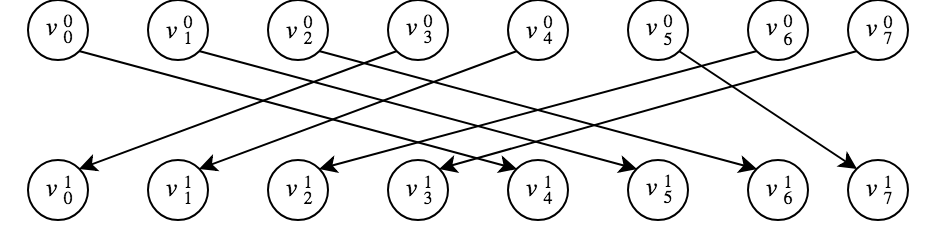
\includegraphics[width=\textwidth]{rp1.png}
	\centering
	\caption{Graf utowrzony z Riffle-Permutation indukowanej przez $B=11100100$.}
\end{figure}

\begin{definition}
	(N-Single-Layer-Riffle-Graph). Niech $V = V^{0} \cup V^{1}$, gdzie $V^{i} = \{ v_{0}^{i},\dots,v_{N-1}^{i} \}$ i niech $B$ będzie słowem binarnym długości $N$. Niech $\pi_{B}$ będzie Riffle-Permutaion indukowaną przez $B$.
	Graf N-Single-Layer-Riffle-Graph (dla parzystego N) zdefiniowany jest jako graf na wierzchołkach $V$ z następującymi krawędziami w zbiorze $E$:
	\begin{itemize}
		\item jedna krawędź: $v_{N-1}^{0} \rightarrow v_{0}^{1}$,
		
		\item $2(N - 1)$ krawędzi: $v_{i-1}^{j} \rightarrow v_{i}^{j}$, dla $i \in [N-1]$ oraz $j \in \{0, 1\}$,
		
		\item $N$ krawędzi: $v_{i}^{0} \rightarrow v_{\pi_{B}(i)}^{1}$, dla $i \in \{0,\dots,N -1\}$,
		
		\item $N$ krawędzi: $v_{i}^{0} \rightarrow v_{\pi_{\overline{B}}(i)}^{1}$, dla $i \in \{0,\dots,N -1\}$.
	\end{itemize}
\end{definition}

\begin{example}
	Kontynuując z danymi z poprzedniego przykładu TODO dodać link,
		$\pi_{\overline{B}} = \bigl( \begin{smallmatrix}
	0 && 1 && 2 && 3 && 4 && 5 && 6 && 7 \\
	0 && 1 && 2 && 4 && 5 && 3 && 6 && 7
	\end{smallmatrix} \bigr) $.
	 8-Single-Layer-Riffle-Graph ukazany jest na Rysynku TODO.
\end{example}

\begin{figure}[h]
	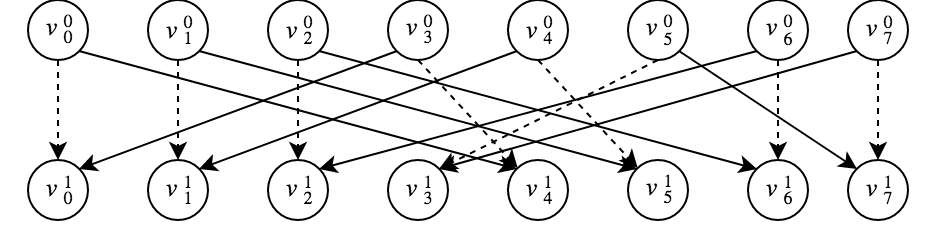
\includegraphics[width=\textwidth]{rp2.png}
	\centering
	\caption{8-Single-Layer-Riffle-Graph dla $B=11100100$ (krawędź $(v_{7}^{0}, v_{0}^{1})$ oraz krawędzie poziome zostały pominięte). Krawędzie dla permutacji $\pi_{B}$ oznaczone są linią ciągłą, a krawędzie dla permutacji $\pi_{\overline{B}}$ oznaczone są linią przerywaną.}
\end{figure}

Od teraz zakładamy, że $N = 2^{g}$.

\begin{definition}
	(N-Double-Riffle-Graph). Niech $V$ oznacza zbiór wierzchołków, a $E$ zbiór krawędzi grafu $G =(V, E)$. Niech $B_{0},\dots,B_{g-1}$ będą wyrazami binarnymi o długości $2^{g}$ każdy.
	N-Double-riffle-Graph jest otrzymywany poprzez ułożenie w stos $2g$ grafów, które spełniają warunki N-Single-Layer-Riffle-Graph. Otrzymany tak graf ma $(2g+1)2^{g}$ wierzchołków $ \{ v_{0}^{0}, \dots , v_{2^{g} - 1}^{0} \} \cup \dots \cup \{ v_{0}^{2g},\dots,v_{2^{g - 1}}^{2g} \} $,
	oraz następujące krawędzie:
	\begin{itemize}
		\item $(2g + 1)2^{g}$ krawędzi: $v_{i-1}^{j} \rightarrow v_{i}^{j}$ dla $i \in [2^{g}-1]$ i $j \in \{0,1,\dots,2^{g} \}$,
		
		\item $2g$ krawędzi: $v_{2^{g} - 1}^{j} \rightarrow v_{0}^{j+1}$ dla $j \in \{0,\dots,2g-1 \} $,
		
		\item $g2^{g}$ krawędzi: $v_{i}^{j-1} \rightarrow v_{\pi_{B_{j}}(i)}^{j}$, dla $i \in \{0,\dots,2^{g} -1\}$ i $j \in [g]$,
		
		\item $g2^{g}$ krawędzi: $v_{i}^{j-1} \rightarrow v_{\pi_{\overline{B}_{j}}(i)}^{j}$, dla $i \in \{0,\dots,2^{g} -1\}$ i $j \in [g]$,
	\end{itemize}
	oraz dla dolnych $g$ warstw, które są symetryczne względem warstwy $g$:
	\begin{itemize}
		\item $g2^{g}$ krawędzi: $v_{i}^{2g - j} \rightarrow v_{\pi_{B_{j}}^{-1}(i)}^{2g -j + 1}$, dla $i \in \{0,\dots,2^{g} -1\}$ i $j \in [g]$,

		\item $g2^{g}$ krawędzi: $v_{i}^{2g - j} \rightarrow v_{\pi_{\overline{B}_{j}}^{-1}(i)}^{2g - j + 1}$, dla $i \in \{0,\dots,2^{g} -1\}$ i $j \in [g]$,
	\end{itemize}

\end{definition}


\begin{definition}
	((N,$\lambda$)-Double-Riffle-Graph). Niech $G_{i}$, $i \in \{ 0,1,\dots,\lambda - 1\}$ będą N-Double-Riffle-Graph. Graf (N,$\lambda$)-Double-Riffle-Graph jest skonstruowany poprzez złączenie wyjść grafu $G_{i}$ do dopowiadających wejść grafu $G_{i+1}$, $i \in \{ 0, 1, \dots, \lambda - 2\}$.
\end{definition}

\subsection{Śledzienie Trajektorii}
Graf jest generowany za pomocą permutacji pseudolosowej $\sigma$.
Ponieważ do generowania grafu potrzebne jest $g$ słów binarnych o długości $2^{g}$, a permutacje zawierają $2^{g}$ elementów, gdzie każdy ma maksymalnie $g$ bitów znaczących, trzeba przekształcić permutację tak, aby otrzymać pożądane dane.
Ta procedura nazwana jest śledzeniem trajektorii (ang. \textit{trace trajectories}).
Niech $B$ będzie macierzą binarną o rozmiarze $2^{g} \times g$, gdzie $j$-ta kolumna jest binarną postacią $\sigma(j) \in [2^{g}-1]$. Macierz $\mathfrak{B} = (\mathfrak{B}_{0},\dots,\mathfrak{B}_{g-1})$ oznaczać będzie transpozycję macierzy $B$, a więc macierz o potrzebnym do generacji grafu rozmiarze $g \times 2^{g}$.

\section{Algorytm}

Procedurę $\mathbf{RiffleScrambler}(pwd, s, g,\lambda)$ można z grubsza przedstawić następująco.

\begin{itemize}
	\item Dla podanej soli $s$ obliczana jest pseudolosowa permutacja $\sigma$ (używając algorytmu inverse Riffle Shuffle).
	
	\item Dla permutacji $\sigma$ tworzona jest macierz $\mathfrak{B} = \mathbf{TraceTrajectories}(B)$.
	
	\item Dla wyrazów binarnych $\mathfrak{B}_{0},\dots,\mathfrak{B}_{g-1}$ generowany jest graf $G$, który jest N-Double-Riffle-Graph. Przypomnijmy, $N = 2 ^ {g}$.
	
	\item Na grafie $G$ zainicjalizowanym wartością $pwd$, oblicze są wartości w ostatnim rzędzie ($v_{0}^{2g+1},\dots,v_{2^{g} - 1}^{2g + 1}$).
	
	\item Wartości z ostatniego rzędu przepisywane są do pierwszego, $v_{i}^{0} = v_{1}^{2g+1}$ dla $i \in \{ 0,\dots,2^{g}-1 \}$, a następnie znów oblicza się wartość ostatnich rzędów. Powtarzane jest $\lambda$ razy.
	
	\item Wartością końcową jest wartość w ostatnim wierzchołku, czyli w $v_{2^{g} - 1}^{2g}$.
\end{itemize}

\begin{example}
	(Generacja (8,1)-Double-Riffle-Graph).
	Skoro $N = 8$, to $g = 3$, ponieważ $N = 2^g$. $\lambda = 1$.
	Niech otrzymaną permutacją $\sigma$ będzie $\bigl( \begin{smallmatrix}
	0 && 1 && 2 && 3 && 4 && 5 && 6 && 7 \\
	5 && 4 && 6 && 3 && 2 && 7 && 0 && 1
	\end{smallmatrix} \bigr) $.
	Zatem binarna postać permutacji $B = \bigl( \begin{smallmatrix}
		1 && 1 && 1 && 0 && 0 && 1 && 0 && 0 \\
		0 && 0 && 1 && 1 && 1 && 1 && 0 && 0 \\
		1 && 0 && 0 && 1 && 0 && 1 && 0 && 1
	\end{smallmatrix} \bigr) $.
	Przeprowadzając śledzenie trajektorii, czyli transponując $B$ otrzymujemy
	$\mathfrak{B} = (\mathfrak{B_0}, \mathfrak{B_1}, \mathfrak{B_2})$, $\mathfrak{B} =\bigl( \begin{smallmatrix}
	1 && 1 && 1 && 0 && 0 && 1 && 0 && 0 \\
	0 && 0 && 1 && 1 && 1 && 1 && 0 && 0 \\
	1 && 0 && 0 && 1 && 0 && 1 && 0 && 1
	\end{smallmatrix} \bigr)^{T} $.
	
	Teraz należy obliczyć permutacje $\pi_{\mathfrak{B_0}},\pi_{\mathfrak{B_1}},\pi_{\mathfrak{B_2}}$:
	
	$$ \pi_{\mathfrak{B_0}}=\bigl( \begin{smallmatrix}
	0 && 1 && 2 && 3 && 4 && 5 && 6 && 7 \\
	4 && 5 && 6 && 0 && 1 && 7 && 2 && 3
	\end{smallmatrix} \bigr), $$
		$$ \pi_{\mathfrak{B_1}}=\bigl( \begin{smallmatrix}
	0 && 1 && 2 && 3 && 4 && 5 && 6 && 7 \\
	0 && 1 && 4 && 5 && 6 && 7 && 2 && 3
	\end{smallmatrix} \bigr), $$
		$$ \pi_{\mathfrak{B_2}}=\bigl( \begin{smallmatrix}
	0 && 1 && 2 && 3 && 4 && 5 && 6 && 7 \\
	4 && 0 && 1 && 5 && 2 && 6 && 3 && 7
	\end{smallmatrix} \bigr). $$
	
	Wygenerowany graf z krawędziami zależnymi od permutacji ukazany jest na ...
	Dodając do nie go krawędzie nie zależne od permutacji, otrzymujemy pełny graf (8,1)-Double-Riffle-Graph.
	
\end{example}


\begin{figure}
		\centering
		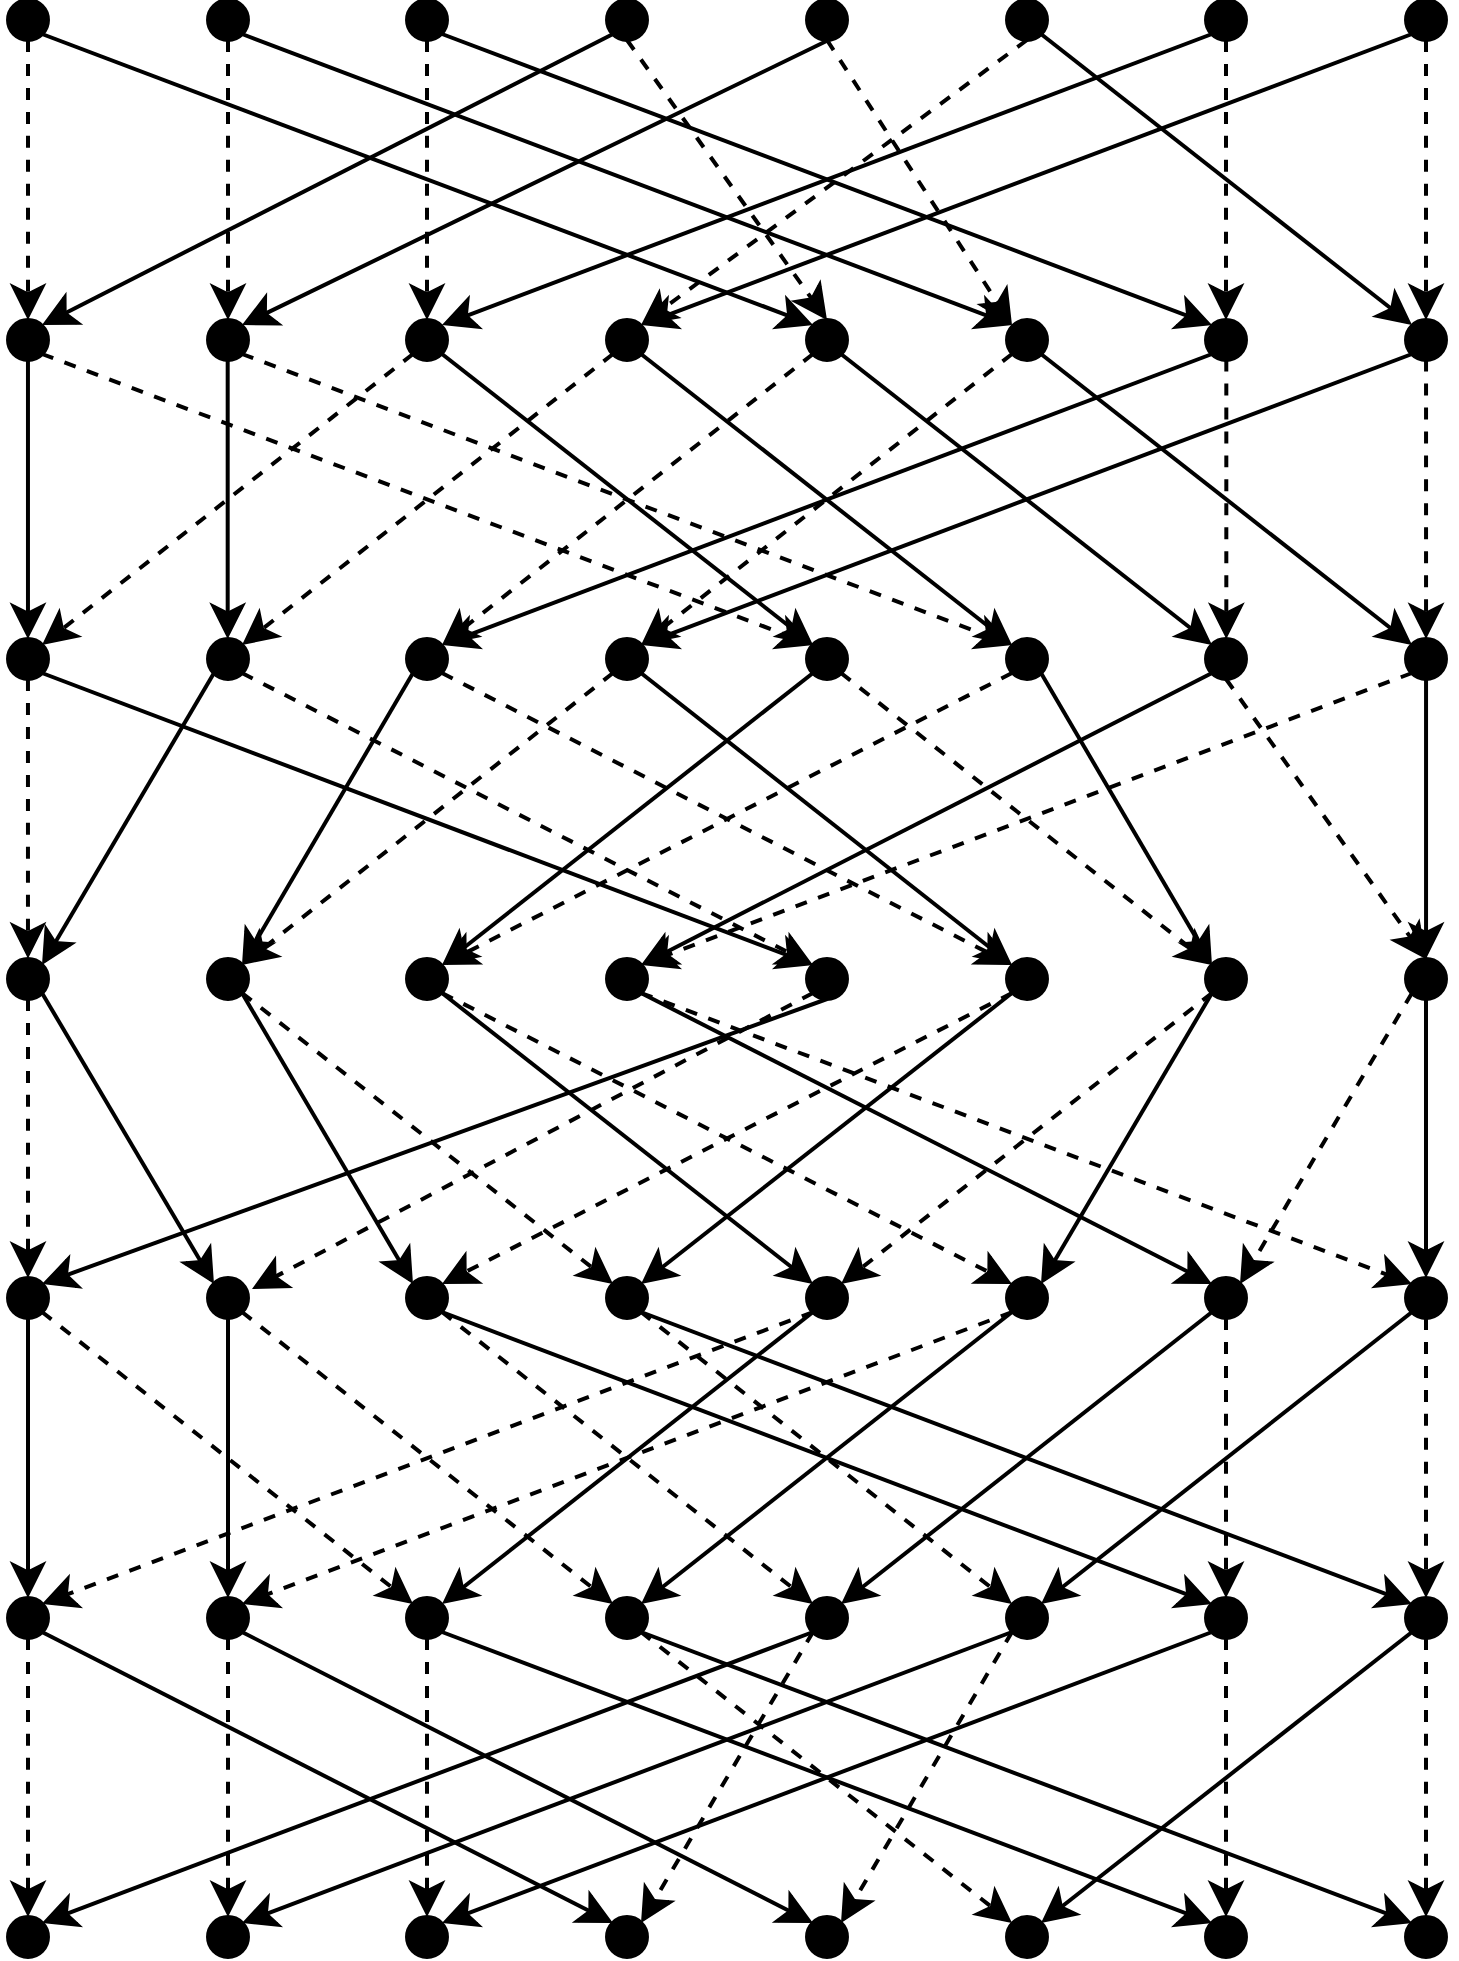
\includegraphics[width=0.7\textwidth]{all_rs1.png}

		\caption{(8,1)-Double-Riffle-Graph (krawiędzie niezależne od permutacji, czyli przekątne oraz krawędzie poziome, zostały pominięte). Krawędzie dla permutacji oznaczone są linią ciągłą, a krawędzie dla permutacji negacji oznaczone są linią przerywaną.}
\end{figure}

\begin{figure}
	\centering
	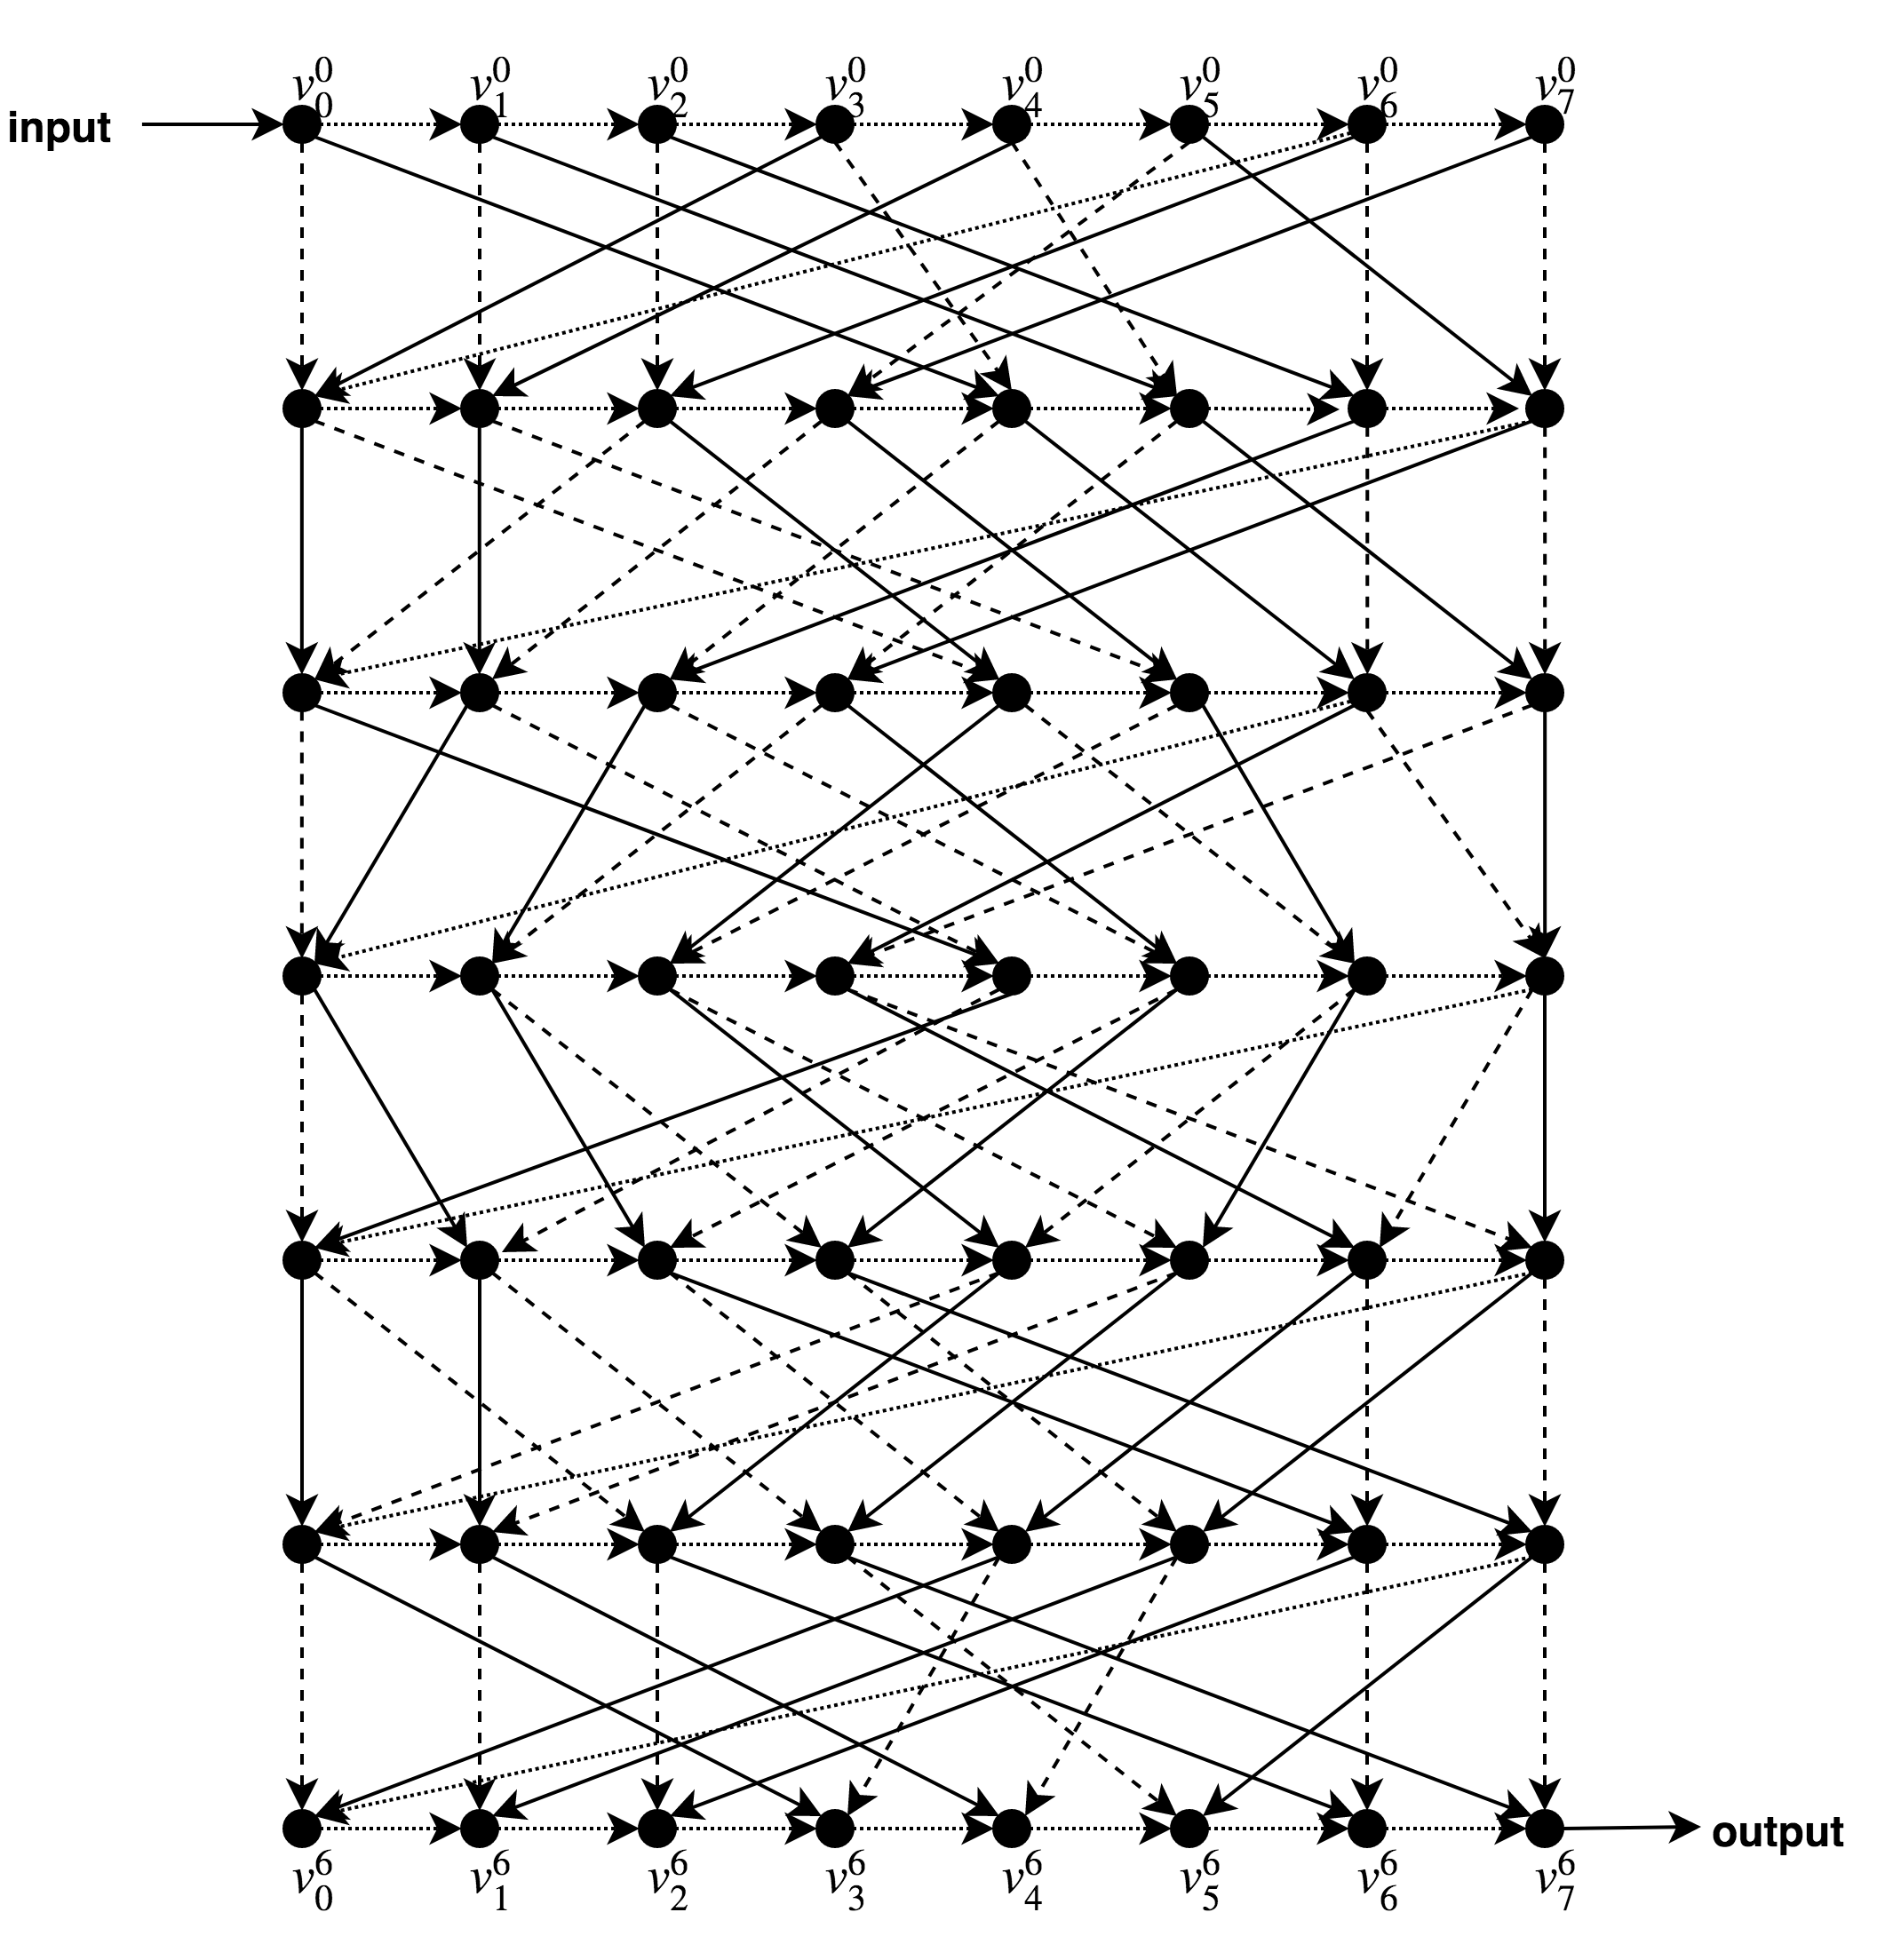
\includegraphics[width=\textwidth]{total_rs.png}
	
	\caption{(8,1)-Double-Riffle-Graph ze wszystkimi krawędziami oraz oznaczeniem wejścia i wyjścia. Krawędzie dla permutacji oznaczone są linią ciągłą, krawędzie dla permutacji negacji oznaczone są linią przerywaną, a krawędzie nie zależne od permutacji oznaczone są liniami kropkowanymi}
\end{figure}




